%% ****** Start of file aiptemplate.tex ****** %
%%
%%   This file is part of the files in the distribution of AIP substyles for REVTeX4.
%%   Version 4.1 of 9 October 2009.
%%
%
% This is a template for producing documents for use with 
% the REVTEX 4.1 document class and the AIP substyles.
% 
% Copy this file to another name and then work on that file.
% That way, you always have this original template file to use.

%\documentclass[aip,graphicx]{revtex4-1}
%\documentclass[aip,reprint]{revtex4-1}

%\usepackage{graphicx}

%\draft % marks overfull lines with a black rule on the right
%\documentclass[pre,aps,floatfix,authordate1-4,twocolumn]{revtex4-1}
%\documentclass[pre,aps,floatfix,authordate1-4]{revtex4-1}

\documentclass[aps,prl,superscriptaddress,twocolumn]{revtex4}



%\documentclass[aps,prl,preprint,groupedaddress]{revtex4}

\usepackage{rotating} 
\usepackage{times}
\usepackage{graphicx}
\usepackage{setspace}
\usepackage{amsmath}
\usepackage{epstopdf}
\usepackage[obeyFinal]{easy-todo}
\usepackage{xr}
\externaldocument{manuscriptSUPPL}
\begin{document}

% Use the \preprint command to place your local institutional report number 
% on the title page in preprint mode.
% Multiple \preprint commands are allowed.
%\preprint{}

\title{NMRlipids III: Lipid-cholesterol interactions in atomistic resolution molecular dynamics simulations} %Title of paper

% repeat the \author .. \affiliation  etc. as needed
% \email, \thanks, \homepage, \altaffiliation all apply to the current author.
% Explanatory text should go in the []'s, 
% actual e-mail address or url should go in the {}'s for \email and \homepage.
% Please use the appropriate macro for the type of information

% \affiliation command applies to all authors since the last \affiliation command. 
% The \affiliation command should follow the other information.

\author{Fernando Favela-Rosales}
\affiliation{Departamento de F\'isica, Centro de Investigaci\'on y de Estudios Avanzados del IPN, Apartado Postal 14-740, 07000 M\'exico D.F., M\'exico}

\author{Peter Heftberger}
%\email[]{samuli.ollila@aalto.fi}
%\homepage[]{Your web page}
%\thanks{}
%\altaffiliation{}
\affiliation{University of Graz}

\author{Matti Javanainen}
\affiliation{Department of Physics, Tampere University of Technology, Tampere, Finland}
\affiliation{University of Helsinki}

\author{Jesper J. Madsen}
\affiliation{Department of Global Health, College of Public Health}
\affiliation{University of South Florida}

\author{Josef Melcr}
\affiliation{Institute of Organic Chemistry and Biochemistry,
Academy of Sciences of the Czech Republic, 
Prague 6, Czech Republic}

\author{Markus Miettinen}
\affiliation{MPI}

\author{O. H. Samuli Ollila}
\email[]{samuli.ollila@helsinki.fi}
%\homepage[]{Your web page}
%\thanks{}
%\altaffiliation{}
\affiliation{Institute of Organic Chemistry and Biochemistry,
Academy of Sciences of the Czech Republic, 
Prague 6, Czech Republic}
\affiliation{Institute of Biotechnology, University of Helsinki}


\author{Georg Pabst}
\affiliation{University of Graz}

\author{Thomas Piggot}
\affiliation{University of Southampton}

% Collaboration name, if desired (requires use of superscriptaddress option in \documentclass). 
% \noaffiliation is required (may also be used with the \author command).
%\collaboration{}
%\noaffiliation

\date{\today}

\begin{abstract}
% insert abstract here
The quantitative quality of lipid-cholesterol interactions in atomistic resolution models will be determined against 
NMR and scattering data.
\end{abstract}

%\pacs{}% insert suggested PACS numbers in braces on next line

\maketitle %\maketitle must follow title, authors, abstract and \pacs

% Body of paper goes here. Use proper sectioning commands. 
% References should be done using the \cite, \ref, and \label commands


%\label{}
\section{Introduction}
Details of intermolecular interactions determine the phase
behaviour and details lateral organization of lipid and bilayers
containing cholesterol \cite{ipsen87}.~\todo{Fix Ole's name among the authors of this paper.}
Formation of lateral heterogeneities \cite{kinnunen91}, lipid rafts \cite{simons97}
and superlattices \cite{somerharju09} in cellular membranes have been
suggested to be driven by interactions between cholesterol
and lipids. While detailed experimental information of these interactions
is relatively sparse, atomistic resolution molecular dynamics simulations
have been widely applied to give detailed explanations of lipid bilayer
lateral organization and lipid-cholesterol interactions \cite{rog14,sodt14,??}.
However, the simulations must reproduce the measured experimental details, such as NMR
order parameters and scattering form factors, to be useful in intepretation
of molecular details in lipid bilayer mixtures.

Simulations qualitatively reproduce the cholesterol condensation effect,
but quantitative comparison to robust experimental data has not been
typically done. This is partly due to the lack of availability of
systematic experimental data sets for the comparison and partly
due to the lack of protocols for validating intermolecular interactions
in lipid bilayer simulations against experiments.
Scattering experiments are more difficult to interpret for
mixed lipid bilayers than for single component bilayers \cite{pan12,Heftberger15,Marquardt15,??},
thus area per molecule values, one of the main quantity used to
compare simulations to experiments, have not been
available for lipid cholesterol mixtures. Systematic experimental
data set for lipid C-H bond order parameters with different cholesterol
concentrations in POPC bilayer has been published only relatively recently \cite{ferreira13}.

In this work we present the experimental scattering form factor
data for POPC-cholesterol mixtures by systematically increasing the
cholesterol concentration, scanning the same concentrations that were previously studied with ssNMR~\cite{ferreira13}.
Our goal is to show that the combination
of systematically measured C--H bond order parameter and scattering form
factor data can be used to validate the quality of lipid--cholesterol
intermolecular interactions in MD simulations. MD simulations can be also
potentially used to give structural interpretation for form factors
measured from mixed systems, which is a major challenge for current methods \cite{pan12,Heftberger15,Marquardt15,??}. 
The approach should be also applicable for mixed lipid bilayers with
other than lipid--cholesterol mixtures.

%Importance of phospholipid cholesterol interactions in cellular membranes
%have been reckognized for long time \cite{??}. Various ideas about 
%lateral heterogeneities driven interactions between cholesterol, phosphatidylcholine
%other other membrane lipids has been proposed \cite{??}. 
%Especially coexistence of liquid-ordered and liquid-disordered phases
%in PC-cholesterol mixtures has been suggested to be important in
%biological lipid membranes \cite{??}. 

%Phase diagram of PC lipid cholesterol systems, including lo-ld coexistence
%can be explained by simple models where cholesterol is assumed to 
%induce order in neighboring lipids \cite{??}. This is important
%achievement in order to understand biomembrane organization. 
%However, also more detailed interactions driving interactions 
%between cholesterol and other membrane lipid molecules are
%often relevant. Several attempts to understand these interactions
%have been made by using classical molecular dynamics simulations \cite{??}.
%These simulations give atomistic resolution information, which not
%directly accessible with any other techinique. However, 
%the simulations often suffer from inaccuracies in force field
%descriptions. Acyl chain region is usually well described in 
%molecular dynamics simulation models, which is not the case for 
%glycerol backbone and headgroup \cite{??}. 
%The same applies to the systems with cholesterol. Practically all simulation
%models qualitatively reproduce the condesing due to cholesterol, observed
%as increase in acyl chain order parameters and decrease of area per molecule.
%However, the some models significantly overestimate the changes in headgroup
%due to the addition of cholesterol \cite{??}. 

%On the other hand, detailed analysis of lateral organization of 
%lipid-cholesterol mixtures reveal significant differences between
%different models. For example, significant angular organization
%of lipids around cholesterol was observed in simulations with Berger
%Höjtje models, while CHARMM36 simulations did not show such behaviour.


Order parameters for C-H bond vectors in lipid bilayer systems, measured
with $^{13}$C or $^{2}$H NMR techniques, give indirect information about the structural
sampling of indidual molecules \cite{ollila16}. The observed increase of
acyl chain order parameters with added cholesterol in simulations and
experiments can be explained by increased trans conformations in acyl chains \cite{ferreira13,??},
which is suggested to play critical role in the phase behaviour of PC-lipid--cholesterol
mixtures \cite{ipsen87}. Consequently, the correct cholesterol ordering effect is
expected to be a necessary condition for a model used to understand lipid--cholesterol
phase behaviour.

\section{Methods}

\subsection{X-ray scattering experiments}

SAXS data on POPC multilamellar vesicles (MLVs) at various cholesterol concentrations
has been measured. Data have been obtained at the EMBL BioSAXS beamline (Hamburg) using 20 keV photons, T = 27$^\circ$C. Data were analyzed in terms of the SDP-GAP model described in Heftberger et al., J. Appl. Cryst. 2013 and Heftberger et al. Biophys. J. 2015. Data from MLVs are a convolute of structure factor (the crystalline lattice) and form factor. By fitting the scattered intensity data we obtain both contributions. Here we posted only form factors (ASCII format). For information on the quality of the fit we also give plots of the fitted intensity data. The electron density profile has been modelled in terms of the SDP model (see papers by Kucerka and coworkers), that is volume distribution functions are modelled by individual Gaussians or error functions. Cholesterol is also accounted for by two Gaussians. This model has been proposed by Jianjun Pan (USF, Tampa, FL), but is to the best of our knowledge not published (see also PhD Thesis by Peter Heftberger). Additional figures show the volume distribution functions and the resulting electron density profiles.

Authors to consult and potentially include in publications using this data: Peter Heftberger (peter.heftberger@gmx.at), Georg Pabst (georg.pabst@uni-graz.at)

\subsection{Molecular dynamics simulations}

Molecular dynamics simulation data was collected using the open collaboration method \cite{botan15}.
Simulated systems are listed in Table \ref{systemsCHOL} and the full simulation
details are given in references or in supplementary material.

\begin{table*}[]
  \centering
  \caption{Simulated lipid bilayers containing cholesterol. The simulation file data sets marked with $^*$ include also part of the trajectory.
    $^a$ The number of lipid molecules
    $^b$ The number of cholesterol molecules
    $^c$ Cholesterol concentration (mol\%)
    $^d$ The number of water molecules
    $^e$ Simulation temperature
    $^f$ The total simulation time
    $^g$ Time frames used in the analysis
    $^h$ Reference link for the downloadable simulation files
    $^i$ Reference for the full simulation details
  }\label{systemsCHOL}
  \begin{tabular}{c c c c c c c c c c c}
    %\hline
    Force field & lipid   & $^a$N$_{\rm l}$ & $^b$N$_{\rm chol}$ &$^c$C$_{\rm CHOL}$  &  $^d$N$_{\rm w}$ & $^e$T (K)  & $^f$t$_{{\rm sim}}$(ns)  & $^g$t$_{{\rm anal}}$ (ns)& $^h$Files  &  $^i$Details\\
    \hline
    Berger-POPC-07~\cite{ollila07a}&   POPC &128 & 0 &0\% & 7290  & 298  & 270 & 240 & [\citenum{bergerFILESpopc}]$^*$ & [\citenum{ferreira15}] \\
    /H\"oltje-CHOL-13~\cite{holtje01,ferreira13}   &    & &  &   &   &  &  &  &  \\
    &   POPC &120 & 8 & 6\% &7290   & 298  & 100 & 80 & [\citenum{bergerFILESpopc7chol}]$^*$ & [\citenum{ferreira13}] \\
    &   POPC &110 & 18& 14\% & 8481  & 298  & 100 & 80 & [\citenum{bergerFILESpopc15chol}]$^*$ & [\citenum{ferreira13}]  \\
    &   POPC &84 & 44 & 34\%  & 6794   & 298  & 100 & 80 & [\citenum{bergerFILESpopc34chol}]$^*$ & [\citenum{ferreira13}] \\
    &   POPC &64 & 64 & 50\% & 10314  & 298  & 100 & 80 & [\citenum{bergerFILESpopc50chol}]$^*$ & [\citenum{ferreira13}] \\
    &   POPC &50 & 78 & 61\% & 5782   & 298  & 100 & 80 & [\citenum{bergerFILESpopc60chol}]$^*$ & [\citenum{ferreira13}] \\
CHARMM36\cite{klauda10,lim12}  & POPC   & 200& 0& 0\% & 9000  & 310  & ? & 100 & [\citenum{charmm36gromacs5chol0-30}]$^*$  &  SI   \\
                               & POPC   & 200& 22& 10\% & 9000  & 310  & ? & 100 & [\citenum{charmm36gromacs5chol0-30}]$^*$  &  SI   \\
                               & POPC   & 200& 50& 20\% & 9000  & 310  & ? & 100 & [\citenum{charmm36gromacs5chol0-30}]$^*$  &  SI   \\
                               & POPC   & 200& 86& 30\% & 9000  & 310  & ? & 100 & [\citenum{charmm36gromacs5chol0-30}]$^*$  &  SI   \\
                               & POPC   & 200& 134& 40\% & 15030  & 310  & 109 & 100 & [\citenum{charmm36gromacs5chol40-50}]$^*$  &  SI   \\
                               & POPC   & 200& 200& 50\% & 18000  & 310  & 109 & 100 & [\citenum{charmm36gromacs5chol40-50}]$^*$  &  SI   \\
Slipids\cite{jambeck12b,jambeck12,jambeck13b}  & POPC   & 200 & 0 & 0\%   & ?  & 310 & ? & 100 & [\citenum{slipidsCHOL0-30T310}]$^*$ & SI  \\
                                               & POPC   & 512 & 0 & 0\%   & 23943  & 310 & 170 & 100 & [\citenum{slipidsCHOL0T298}]$^*$ & SI  \\
                                               & POPC   & 200 & 22 & 10\% & ?  & 310 & ? & 100 & [\citenum{slipidsCHOL0-30T310}]$^*$ & SI  \\
                                               & POPC   & 200 & 50 & 20\% & ?  & 310 & ? & 100 & [\citenum{slipidsCHOL0-30T310}]$^*$ & SI  \\
                                               & POPC   & 200 & 86 & 30\% & ?  & 310 & ? & 100 & [\citenum{slipidsCHOL0-30T310}]$^*$ & SI  \\
                                               & POPC   & 358 & 154 & 30\% & 21183  & 298 & 170 & 100 & [\citenum{slipidsCHOL30T298}]$^*$ & SI  \\
                                               & POPC   & 200 & 134 & 40\% & ?  & 310 & 109 & 100 & [\citenum{slipidsCHOL40-50T310}]$^*$ & SI  \\
                                               & POPC   & 200 & 200 & 50\% & ?  & 310 & 109 & 100 & [\citenum{slipidsCHOL40-50T310}]$^*$ & SI  \\
                                               & POPC   & 256 & 256 & 50\% & 20334  & 298 & 170 & 100 & [\citenum{slipidsCHOL50T298}]$^*$ & SI  \\ 
     MacRog\cite{kulig15b}     & POPC   & 128 & 0 & 0\% & 6400  & 310 & 400 & 200 & [\citenum{macrogCHOLfiles}]$^*$ & [\citenum{botan15}] \\ 
                          & POPC   & 114  & 14 & 11\% & 6400  & 310  & 400 & 200 & [\citenum{macrogCHOLfiles}]$^*$ & [\citenum{botan15}]    \\
                          & POPC   & 72   & 56 &  44\% & 6400  & 310  & 400 & 200 & [\citenum{macrogCHOLfiles}]$^*$ & [\citenum{botan15}]    \\
                             & POPC   & 64  & 64 & 50\% & 6400  & 310  & 400 & 200 & [\citenum{macrogCHOLfiles}]$^*$ & [\citenum{botan15}]    \\
                             & POPC   & 56   & 72 & 56\% & 6400  & 310  & 400 & 200 & [\citenum{macrogCHOLfiles}]$^*$ & [\citenum{botan15}]    \\
     Lipid14\cite{walker14,walker15}     & POPC   & 120 & 8 & 6\% &  3968 & 303 & 200 & 200 & [\citenum{lipid14sys1}]$^*$ & SI \\ 
                          & POPC   & 108  & 20  & 16\% & 3968  & 303  & 200 & 200 & [\citenum{lipid14sys2}]$^*$ & SI    \\
                          & POPC   &  84  & 44 &  34\% & 3968  & 303  & 200 & 200 & [\citenum{lipid14sys3}]$^*$ & SI    \\
                             & POPC   & 64  & 64 & 50\% & 3968  & 303  & 200 & 200 & [\citenum{lipid14sys4}]$^*$ & SI    \\
                             & POPC   &  52  & 76 & 59\% & 3968  & 303  & 200 & 200 & [\citenum{lipid14sys5}]$^*$ & SI    \\
\end{tabular}
\end{table*} 





\clearpage

\section{Results and Discussion}

\subsection{Monitoring molecular interactions between POPC and cholesterol in lipid bilayer using NMR and MD simulations}

Addition of cholesterol substantially increases the acyl chain C-H order parameters in PC lipid bilayers (Fig. \ref{OrderParametersCHOL}),
which can be explained by increased trans conformations in acyl chains \cite{ferreira13,??}.
%Acyl chain order parameters for pure 1-palmitoyl-2-oleoylphosphatidylcholine (POPC) bilayer
%and mixture with 50 mol\% of cholesterol from different simulations and experiments
%are shown in Fig. \ref{OrderParametersCHOL}.
The absolute values of order parameters of sn-1 chain from $^{13}$C NMR experiments \cite{ferreira13}
exhibit approximately linear increase with cholesterol up to equimolar mixture (Fig. \ref{slopes}), which is expected because
phase separation is not observed for this mixture \cite{ionova12,ferreira13}.
%thus the intermolecular interactions are expected to have maximum effect in equimolar mixture.
\begin{figure*}[]
  \centering
  \includegraphics[width=17.2cm]{../FIGS/OrderParametersCHOL.eps}
  \caption{\label{OrderParametersCHOL}
    Order parameters from simulations and experiments for acyl chains of  1-palmitoyl-2-oleoylphosphatidylcholine (POPC).
  }
  \todo{Lipid14 results?} 
\end{figure*}

Experimental acyl chain order parameters of pure POPC lipid bilayers
are well reproduced by most force fields (Fig. \ref{OrderParametersCHOL}),
except for the C$_2$ carbon in {\it sn}-1 chain,
which is typically the case in the state of the art lipid force fields (for review see \cite{ollila16}).
%This is also mainly observed in the data
%presented here, except that
However, the order parameters in the beginning of {\it sn}-1 chain are underestimated in the
MACROG simulation and CHARMM36 simulations slightly overestimates the order parameters, also when
used with other than Gromacs simulation packages (section \ref{CHARMMprograms} in the supplementary information).
The absolute values of {\it sn}-1 acyl chain order parameters exhibit approximately linear increase upon addition
of cholesterol also in simulations below equimolar mixture (Figs. \ref{slopesberger}-\ref{slopesslipids310K}).
However, the slope of the increase (Fig. \ref{OrderParametersCHOLchanges}) and order parameters
in equimolar mixtures (Fig. \ref{OrderParametersCHOL}) are overestimated by all force fields.
%For Berger/H\"oltje and MACROG models the overestimation is significant,
%while less severe for CHARMM36 and Slipid models.
The overestimation of order parameters observed in CHARMM without cholesterol and in all force fields
with cholesterol is smaller than the contribution by undulations in large simulations (section \ref{undulations} in the supplementary information).
\begin{figure}[]
  \centering
  \includegraphics[width=8cm]{../FIGS/slopes.eps}
  \caption{\label{OrderParametersCHOLchanges}
    Slopes of order parameters as a function of cholesterol.
  }
\end{figure}

\todo{Also experimental cholesterol order parameters are available. Maybe these should be calculated from simulations as well.}

\subsection{Lipid bilayer dimensions and density profiles as a function of cholesterol}

Lipid bilayer dimensions can be experimentally accessed by measuring X-ray scattering
form factor, which is related to the electron density along membrane normal
via Fourier transformation \cite{pan12,Heftberger15,Marquardt15,ollila16,??}.
%methods and have been widely used to validate lipid bilayer simulations \cite{ollila16,??}. 
The form factor can be translated to density profiles, 
%While sophisticated models are applied to extract
area per lipids and bilayer thickness using SDP model or its combination with MD simulations  \cite{pan12,Heftberger15,Marquardt15,??}.
Sophisticated approaches for single component lipid bilayers are available \cite{??},
but multicomponent systems are more difficult to interpret \cite{pan12,Heftberger15,Marquardt15,??}.
%In such case the validation can be done by comparing directly measurable form factors between
%simulations and experiments. If simulation reproduces the form factor, it can be also
%used to interpret the experiments.

State of the art force fields give good agreement with experimental form factors for
pure POPC lipid bilayers \cite{??}, which is the case also here, except for the Berger
simulation (Fig.~\ref{FormFactors}).
%The form factors from different simulation models with
%different cholesterol concentrations are compared to experimental data in Fig.~\ref{FormFactors}. \\
Upon addition of cholesterol, the third minima in form factor systemically decreases from $\sim$0.42 to $\sim$0.32
%Cholesterol induced changes in lipid packing, thickness and density profiles are suggested
%to be relevant, for example, for membrane protein interactions and cellular membrane
%lateral organization \cite{??}. Experimental and simulation studies show that
%the cholesterol induces the so called ''condensing effect'', i.e. acyl chain ordering
%increases the membrane thickness and
%reduces the area per molecule in lipid bilayers \cite{??}.
This may be related to the reduced area per molecule upon addition of cholesterol (Fig. \ref{apls}).
%, showing the area per PC headgroups and per
%total number of molecules as a function of cholesterol concentration from different
%models.
The area per total amount of molecules decreas with cholesterol in all simulations, partly
due to the smaller area covered by the cholesterol than lipids, but also because
lipids ordered by cholesterol require less space. Due to the latter effect,
the area per PC headgroup does not essentially increase up to the addition of
$\sim$15 mol\% of cholesterol. 
\begin{figure}[]
 \centering
 \includegraphics[width=8cm]{../FIGS/FormFactors.eps}
 \caption{\label{FormFactors}
   Form factors from simulations and experiments.
 }
 \todo{Details about form factor calculation code is discussed in issues
   https://github.com/NMRLipids/MATCH/issues/56 and https://github.com/NMRLipids/MATCH/issues/50.
   Once the code is finalized, we should recalculate and check the form factors.
   CURRENTLY, 10\%-40\% cholesterol concetrations are calculated with a code which gives possibly incorrect
   heigths for the maxima.
 } \\
 \todo{The y-axis scale cannot be explicitly measured in experiments.
   Therefore, the y-axis of the experimental form factor is typically scaled to match with simulations.
   This currently not done, because we have several simulations which give inequal form factors, and therefore
   it is not clear against which simulation results we should scale the experimental results.
   I have created a issue for this discussion: https://github.com/NMRLipids/NmrLipidsCholXray/issues/18
 } \\
 \todo{Not all experimental and simulation data is here (maybe?).}
\end{figure}
\begin{figure}[]
  \centering
  \includegraphics[width=8cm]{../FIGS/apls.eps}
  \caption{\label{apls}
    Area per molecules calculated from different simulation models
    as a function of cholesterol concentration. The solid symbols are area per
    total amount of molecules (chol+PC) and the empty symbols area per PC headgroups.
    Top figure shows absolute values and bottom figure shows changes respect
    to pure lipid system.
  }
\end{figure}

Visual inspection of form factors (Fig. \ref{FormFactors}) and quantitative quality estimation (Fig. \ref{FormFactorsFITNESS})
suggests that the Berge/Holtje force field gives the best agreement with experiments with large
cholesterol concentration. This is surprising because the same model overestimated acyl chain
order parameter increase upon addition of cholesterol more than CHARMM36 or Slipids simulations
(Figs. \ref{OrderParametersCHOL} and \ref{OrderParametersCHOLchanges}).
The Berger/Holtje model also exhibits the most pronounced decrease in the area per molecule
upon addition of cholesterol (Fig. \ref{alps}).
On the other hand, the electron density profiles from Berger/Holtje simulations are closer
to the result from the SDP model then other MD simulation models for both pure POPC bilayer
and equimolar POPC/cholesterol mixture, especially in the middle of the bilayer
where SDP model gives substantially lower density than MD simulations (Fig. \ref{densities}).
Therefore, the good quality of form factor Berger/Holtje model with large amounts of cholesterol
may rather indicate the importance of this low electron density in the bilayer center,
rather than better quality of lipid-cholesterol interactions in this model.
\begin{figure}[]
  \centering
  \includegraphics[width=8cm]{../FIGS/FFfitness.eps}
  \caption{\label{FormFactorsFITNESS}
    Fitness of form factors between simulations and experiments.
  }
\end{figure}

\begin{figure}[]
  \centering
  \includegraphics[width=8cm]{../FIGS/densitiesEXTREMES.eps}
  \caption{\label{densities}
    Electron density profiles from MD simulations and SDP model.
  }
\end{figure}


\section{Presenting the quality of lipid bilayer MD simulation with binary mixtures}  

All the tested MD simulation models qualitatively reproduced experimentally observed condenced and
ordering effects of cholesterol. However, the acyl chain ordering was overestimated and quality
of form factors reduced with increasing amount of cholesterol. Although the biological importance
of these details is unclear, overestimated ordering may promote formation of liquid ordered phases and
inaccuate form factors complicate interpretation of scattering experiment with MD simulations.
Therefore, MD simulation force fields correctly reproducing the order effects upon addition of the
cholesterol would be invaluable.

To facilitate the comparison of the quality of complex lipid bilayers,
we introduce the quantitative quality measures which measure the quality of
intermolecular interactions in binary lipid bilayers from different perspectives.
The simple difference between experimental and simulated C-H bond order parameters
give a very detailed picture about the quality of molecular conformations in all
positions of lipid bilayer (Fig. \ref{OrderParametersCHOLfitness}).
However, complexity of such presentation increases with increasing amount of data
and it may be hard to present in practical format readable for human or machine.
Using root mean square deviation across regions in the molecule simplifies the presentation,
but compromizes the spatial resolution. Here, we divide the lipid into headgroup, glycerol
backbone, sn-1 and sn-2 chains to present quality of binary lipid bilayer in more convenient
format (Fig. \ref{OrderParametersCHOLfitness}).
\todo{Discussion to be finished once we have the fitness function defined.}

\begin{figure*}[]
  \centering
  \includegraphics[width=17.2cm]{../FIGS/OrderParametersCHOLfitness.eps}
  \caption{\label{OrderParametersCHOLfitness}
    Difference between order parameters from simulations and experiments for acyl chains of  1-palmitoyl-2-oleoylphosphatidylcholine (POPC).
  }
\end{figure*}




\section{Conclusions}

%Cholesterol ordering effect is overestimated in Berger/Holtje and MacRog models.
%Slight overestimation is observed also in CHARMM36 and Slipid models, but more
%careful analysis is required to conclude if this is significant or not.



% Tables may be be put in the text as floats.
% Here is an example of the general form of a table:
% Fill in the caption in the braces of the \caption{} command. Put the label
% that you will use with \ref{} command in the braces of the \label{} command.
% Insert the column specifiers (l, r, c, d, etc.) in the empty braces of the
% \begin{tabular}{} command.
%
% \begin{table}
% \caption{\label{} }
% \begin{tabular}{}
% \end{tabular}
% \end{table}

% If you have acknowledgments, this puts in the proper section head.
\begin{acknowledgments}
JJM thanks the Amber community (Benjamin Madej from the Walker lab and Callum Dickson from the Gould lab) for technical assistance related to the lipid14 force field parameters.
\end{acknowledgments}

\bibliography{refs.bib}

%\newpage
%\section{APPENDIX: The NMR results reported by Tiago Ferreira}

\listoftodos

\end{document}
%
% ****** End of file aiptemplate.tex ******
